\documentclass[11pt]{article}
\usepackage[margin=1in]{geometry}
\usepackage{amsmath, amssymb, amsthm}
\usepackage{algorithm, algpseudocode}
\usepackage{graphicx}
\usepackage{xcolor}
\usepackage{listings}
\usepackage{hyperref}
\usepackage{booktabs}
\usepackage{float}

\definecolor{codegreen}{rgb}{0.2,0.6,0.2}
\definecolor{codered}{rgb}{0.7,0.15,0.15}
\definecolor{codegray}{rgb}{0.4,0.4,0.4}
\definecolor{codebg}{rgb}{0.97,0.97,0.97}

\lstset{
  language=R,
  basicstyle=\ttfamily\small,
  keywordstyle=\color{codered}\bfseries,
  commentstyle=\color{codegray}\itshape,
  stringstyle=\color{codegreen},
  backgroundcolor=\color{codebg},
  frame=single,
  rulecolor=\color{codegray!40},
  numbers=left,
  numberstyle=\tiny\color{codegray},
  breaklines=true,
  columns=fullflexible,
  showstringspaces=false,
  tabsize=2,
  xleftmargin=1.5em,
  framexleftmargin=1em,
}

\newcommand{\R}{\textsf{R}}

\title{Importance Sampling: Theory and Implementation}
\author{Adam Kurth \\ PHP 2530 --- Bayesian Statistics}
\date{Spring 2026}

\begin{document}
\maketitle

% ----------------------------------------------------------------
\section{Motivation}

Suppose we want to compute the expectation of some function~$h$ with respect to a target distribution~$p$:
\[
  \mu = E_p[h(X)] = \int h(x)\,p(x)\,dx.
\]
In many Bayesian problems, $p$ is a posterior that is difficult or impossible to sample from directly.  Even when we \emph{can} sample from~$p$, the integrand $h(x)\,p(x)$ may have most of its mass in a region that the sampler rarely visits (a \textbf{rare-event} problem), making naive Monte Carlo hopelessly inefficient.

Importance sampling (IS) solves both problems by drawing from a different, easier distribution~$q$ (the \textbf{proposal} or \textbf{importance distribution}) and correcting for the mismatch via \textbf{importance weights}.  Unlike rejection sampling, IS uses \emph{every} draw---nothing is thrown away---and it does not require the bounding constant~$c$.

% ----------------------------------------------------------------
\section{The Algorithm}

\subsection{Core Identity}

For any density~$q$ with $q(x) > 0$ whenever $h(x)\,p(x) \neq 0$, we can write
\[
  \mu = \int h(x)\,p(x)\,dx
      = \int h(x)\,\frac{p(x)}{q(x)}\,q(x)\,dx
      = E_q\!\left[h(X)\,\frac{p(X)}{q(X)}\right].
\]
The ratio $w(x) = p(x)/q(x)$ is the \textbf{importance weight} (also called the \textbf{likelihood ratio} or \textbf{Radon--Nikodym derivative}).

\subsection{Unnormalized Estimator}

If $p(x)$ is a proper, normalized density, the Monte Carlo estimator is immediate.

\begin{algorithm}[H]
\caption{Importance Sampling (unnormalized)}
\label{alg:is-unnorm}
\begin{algorithmic}[1]
\For{$i = 1, \ldots, N$}
  \State Draw $X^{(i)} \sim q$
  \State Compute weight $w^{(i)} = p(X^{(i)}) / q(X^{(i)})$
\EndFor
\State \Return $\hat{\mu}_N = \dfrac{1}{N}\displaystyle\sum_{i=1}^{N} w^{(i)}\,h(X^{(i)})$
\end{algorithmic}
\end{algorithm}

By the law of large numbers, $\hat{\mu}_N \to \mu$ almost surely as $N \to \infty$.

\subsection{Self-Normalized Estimator}

In Bayesian settings, $p(x)$ is often known only up to a normalizing constant: $p(x) = c\,\tilde{p}(x)$ where $c$ is unknown.  Computing $w^{(i)} = \tilde{p}(X^{(i)})/q(X^{(i)})$ gives \emph{unnormalized} weights.  The \textbf{self-normalized} (or \textbf{ratio}) estimator resolves this:
\[
  \tilde{\mu}_N = \frac{\sum_{i=1}^{N} w^{(i)}\,h(X^{(i)})}{\sum_{i=1}^{N} w^{(i)}}
               = \sum_{i=1}^{N} \tilde{w}^{(i)}\,h(X^{(i)}),
\]
where $\tilde{w}^{(i)} = w^{(i)} / \sum_j w^{(j)}$ are the \textbf{normalized importance weights}.  This estimator is biased but consistent, and is the form most commonly used in practice (BDA3, Section~10.4).

\subsection{Why It Works}

\paragraph{Unbiasedness (unnormalized case).}
Since $X^{(i)} \sim q$,
\[
  E_q\!\left[\frac{1}{N}\sum_{i=1}^N w^{(i)} h(X^{(i)})\right]
  = E_q\!\left[\frac{p(X)}{q(X)} h(X)\right]
  = \int h(x)\,\frac{p(x)}{q(x)}\,q(x)\,dx
  = \int h(x)\,p(x)\,dx
  = \mu.
\]

\paragraph{Variance.}
The variance of the unnormalized estimator is
\[
  \mathrm{Var}_q(\hat{\mu}_N) = \frac{1}{N}\,\mathrm{Var}_q\!\left[\frac{p(X)}{q(X)}\,h(X)\right]
  = \frac{1}{N}\int \left(\frac{p(x)}{q(x)}\,h(x) - \mu\right)^{\!2} q(x)\,dx.
\]
This variance is \textbf{small} when $q$ is roughly proportional to $|h(x)|\,p(x)$, and \textbf{large} (possibly infinite) when $q$ has lighter tails than $p$ in regions where $|h(x)\,p(x)|$ is appreciable.  This is the central design principle of IS: \emph{the proposal should cover the target where the integrand matters}.

\paragraph{The optimal proposal.}
In theory, the zero-variance IS estimator uses
\[
  q^*(x) = \frac{|h(x)|\,p(x)}{\int |h(x)|\,p(x)\,dx}.
\]
This is impractical (computing the denominator is the very integral we seek), but it tells us that $q$ should place mass where $|h(x)\,p(x)|$ is large.

% ----------------------------------------------------------------
\section{Effective Sample Size}

When some weights are much larger than others, a few samples dominate the estimator.  The \textbf{effective sample size} (ESS) quantifies this:
\[
  \mathrm{ESS} = \frac{\left(\sum_{i=1}^N w^{(i)}\right)^2}{\sum_{i=1}^N \left(w^{(i)}\right)^2}.
\]
When all weights are equal ($q = p$), $\mathrm{ESS} = N$.  When one weight dominates, $\mathrm{ESS} \approx 1$.  A useful rule of thumb: if $\mathrm{ESS}/N$ is small (say $< 0.1$), the proposal is a poor match for the target.

% ----------------------------------------------------------------
\section{Implementation in \R}

The companion script \texttt{importance-sampling.r} demonstrates three examples with five figures.

\subsection{Example 1: $\mathrm{Beta}(5,2)$ via $\mathrm{Uniform}(0,1)$}

\paragraph{Setup.}
The target is $p(x) = \mathrm{Beta}(x;\,5,2)$ and we want $E_p[X] = a/(a+b) = 5/7 \approx 0.7143$.  The proposal is $q(x) = \mathrm{Uniform}(0,1)$, giving weights $w(x) = p(x)/q(x) = p(x)$ since $q(x) = 1$.

\begin{lstlisting}
a <- 5; b <- 2
true_mean <- a / (a + b)
N <- 10000
x_q <- runif(N)
w_raw <- dbeta(x_q, a, b) / dunif(x_q)
w_norm <- w_raw / sum(w_raw)
\end{lstlisting}

\paragraph{Estimators.}
We compute both the unnormalized and self-normalized IS estimates:
\begin{lstlisting}
IS_unnorm <- mean(w_raw * x_q)
IS_selfnorm <- sum(w_norm * x_q)
\end{lstlisting}

Both converge to the true mean.  The naive Monte Carlo estimate $\bar{x} = \frac{1}{N}\sum x_i \approx 0.50$ is wrong because it computes $E_q[X]$, not $E_p[X]$.

\paragraph{Figure~\ref{fig:mechanics}: IS mechanics.}
Panel~(a) overlays $p(x)$ and $q(x)$, showing the mismatch the weights must correct.  Panel~(b) plots the weight function $w(x) = p(x)/q(x)$: samples near $x = 1$ are upweighted because $p$ has more mass there than~$q$.  Panel~(c) shows the raw weights as a scatter plot, and Panel~(d) displays the self-normalized weights as a discrete approximation to $p$.

\begin{figure}[H]
  \centering
  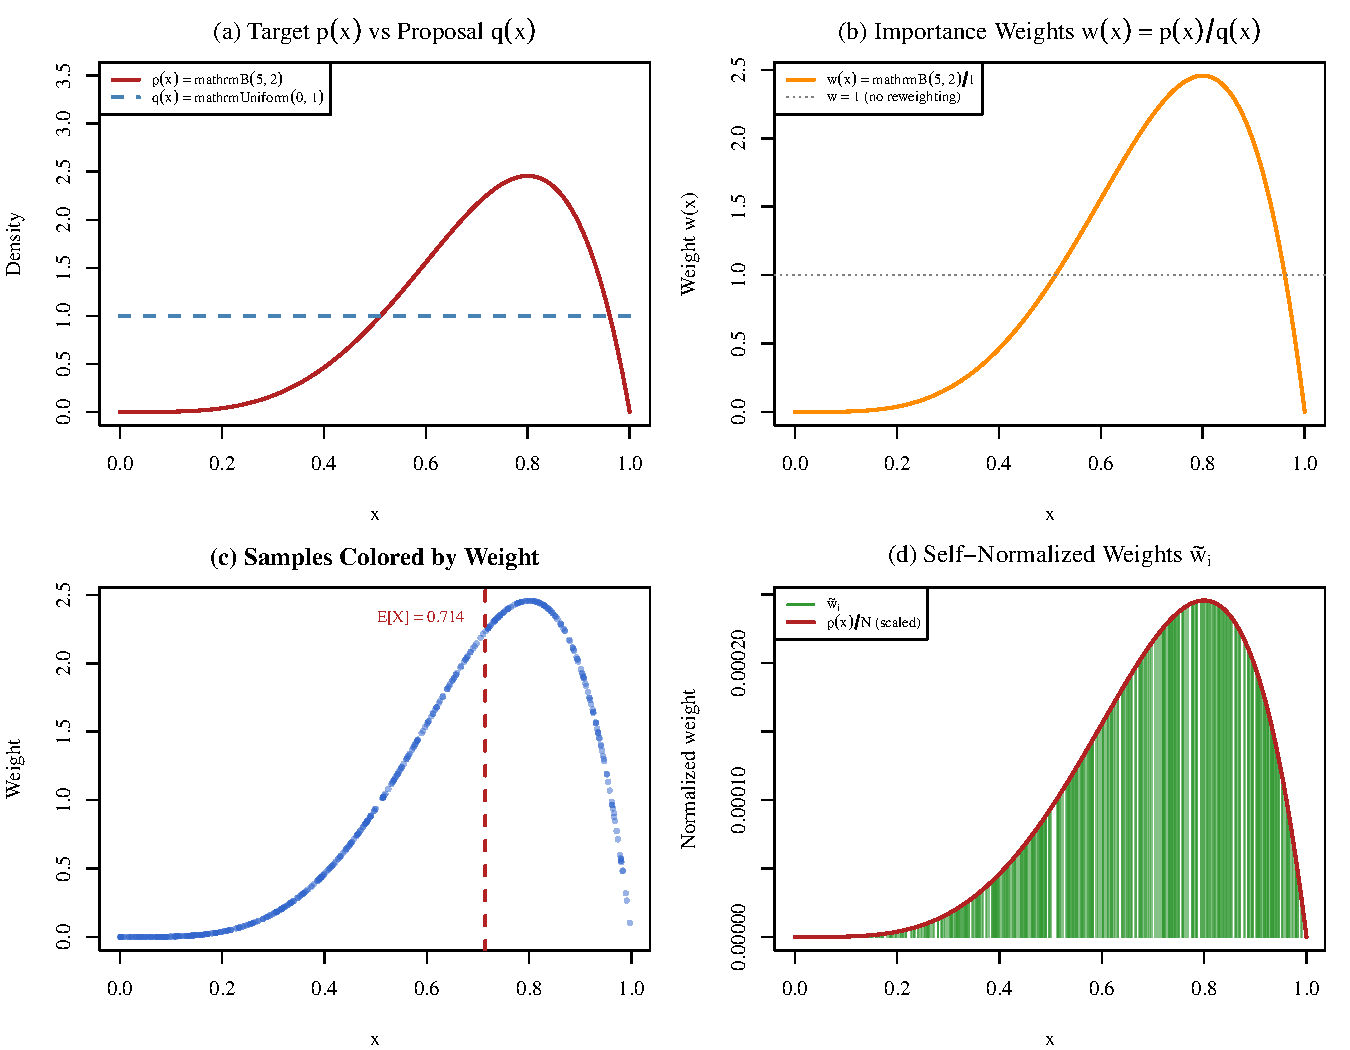
\includegraphics[width=\textwidth]{plots/fig_is_mechanics.pdf}
  \caption{%
    \textbf{(a)}~Target $p(x) = \mathrm{Beta}(5,2)$ vs.\ proposal $q(x) = \mathrm{Uniform}(0,1)$.
    \textbf{(b)}~Importance weight function $w(x)=p(x)/q(x)$; samples near $x=1$ receive high weight.
    \textbf{(c)}~Scatter of samples vs.\ their weights.
    \textbf{(d)}~Self-normalized weights form a discrete approximation to $p(x)$.
  }
  \label{fig:mechanics}
\end{figure}

% ----------------------------------------------------------------
\subsection{Example 2: Rare-Event Estimation---$P(X > 4)$}

\paragraph{Setup.}
For $X \sim N(0,1)$, the tail probability $P(X > 4) \approx 3.17 \times 10^{-5}$ is extremely small.  Direct Monte Carlo with $M = 50{,}000$ samples will often produce \emph{zero} hits.  IS with a shifted proposal $q(x) = N(4,1)$ places samples directly in the tail.

\begin{lstlisting}
mu_q <- 4
x_is <- rnorm(M, mean = mu_q, sd = 1)
w_tail <- dnorm(x_is) / dnorm(x_is, mean = mu_q, sd = 1)
IS_tail <- mean(w_tail * (x_is > threshold))
\end{lstlisting}

\paragraph{Figure~\ref{fig:tail}: Rare-event estimation.}
Panel~(a) shows why direct MC fails: the shaded region under $\phi(x)$ to the right of $x=4$ contains negligible probability, so random $N(0,1)$ draws almost never land there.  The shifted $N(4,1)$ proposal places its center right at the threshold.  Panel~(b) compares convergence: IS stabilizes quickly around the true value, while direct MC remains stuck at zero for most sample sizes.

\begin{figure}[H]
  \centering
  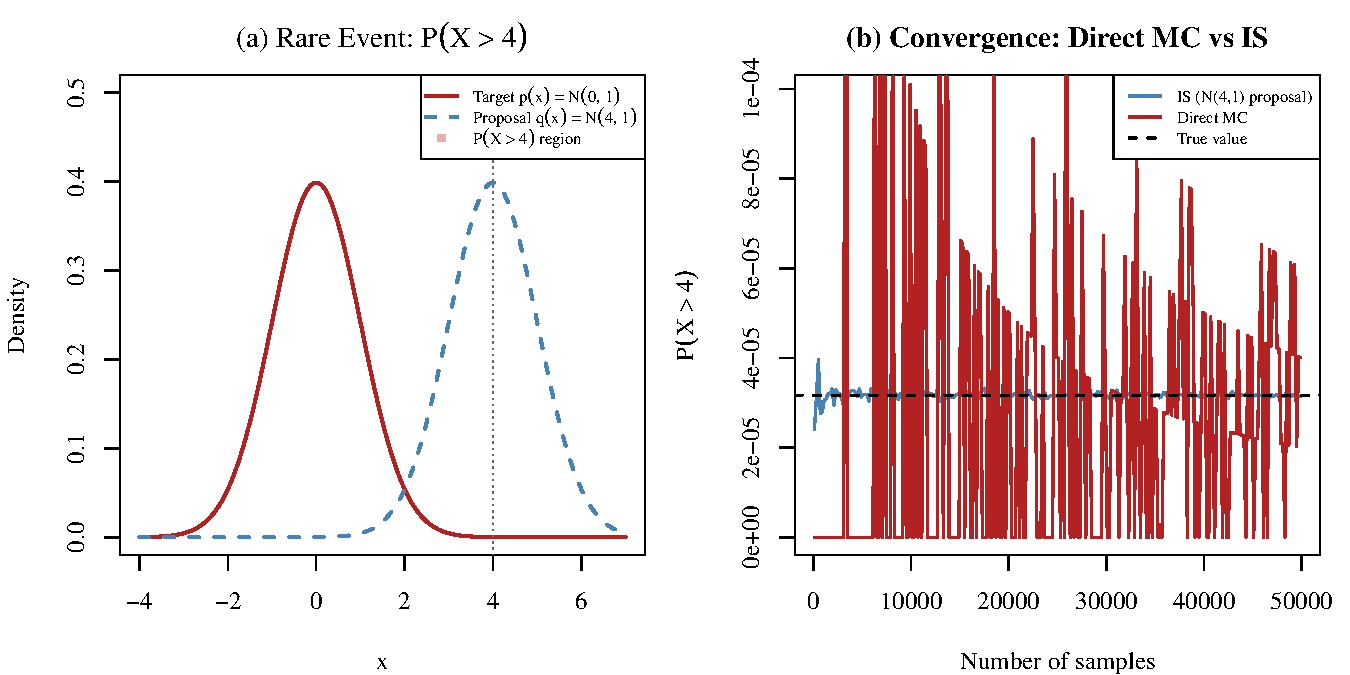
\includegraphics[width=\textwidth]{plots/fig_is_tail.pdf}
  \caption{%
    \textbf{(a)}~The standard normal target (red) has negligible mass beyond $x=4$; the shifted $N(4,1)$ proposal (blue) covers this region.
    \textbf{(b)}~IS converges rapidly to the true probability, while direct MC rarely produces any hits.
  }
  \label{fig:tail}
\end{figure}

% ----------------------------------------------------------------
\subsection{Example 3: Good vs.\ Bad Proposals}

\paragraph{Setup.}
We estimate $E[X^2] = 1$ for $X \sim N(0,1)$ using two proposals:
\begin{itemize}
  \item \textbf{Good}: $q(x) = t_3(x)$---heavier tails than $N(0,1)$, centered at zero.  This ensures $w(x) = \phi(x)/t_3(x)$ is bounded and well-behaved.
  \item \textbf{Bad}: $q(x) = N(3,\,0.5^2)$---shifted far from the target's center and too narrow.  Most samples fall in a region where $p$ has little mass, producing many near-zero weights and a few enormous ones.
\end{itemize}

Over 200 replications, the $t_3$ proposal gives low-variance estimates tightly concentrated around 1, while the $N(3,\,0.25)$ proposal yields wildly unstable estimates.

\begin{lstlisting}
# Good proposal: t_3
x_g <- rt(K, df = 3)
w_g <- dnorm(x_g) / dt(x_g, df = 3)

# Bad proposal: N(3, 0.25)
x_b <- rnorm(K, mean = 3, sd = 0.5)
w_b <- dnorm(x_b) / dnorm(x_b, mean = 3, sd = 0.5)
\end{lstlisting}

\paragraph{Figure~\ref{fig:proposal}: Proposal comparison.}
Panel~(a) overlays the target and both proposals.  Panel~(b) shows the weight distribution for the good proposal: weights are concentrated near their mean with no extreme outliers.  Panel~(c) shows the \emph{log}-scale weight distribution for the bad proposal: most weights are astronomically small, with a handful of extreme values driving the entire estimate.  Panel~(d) displays boxplots of the IS estimates over 200 replications---the bad proposal has enormous variance.

\begin{figure}[H]
  \centering
  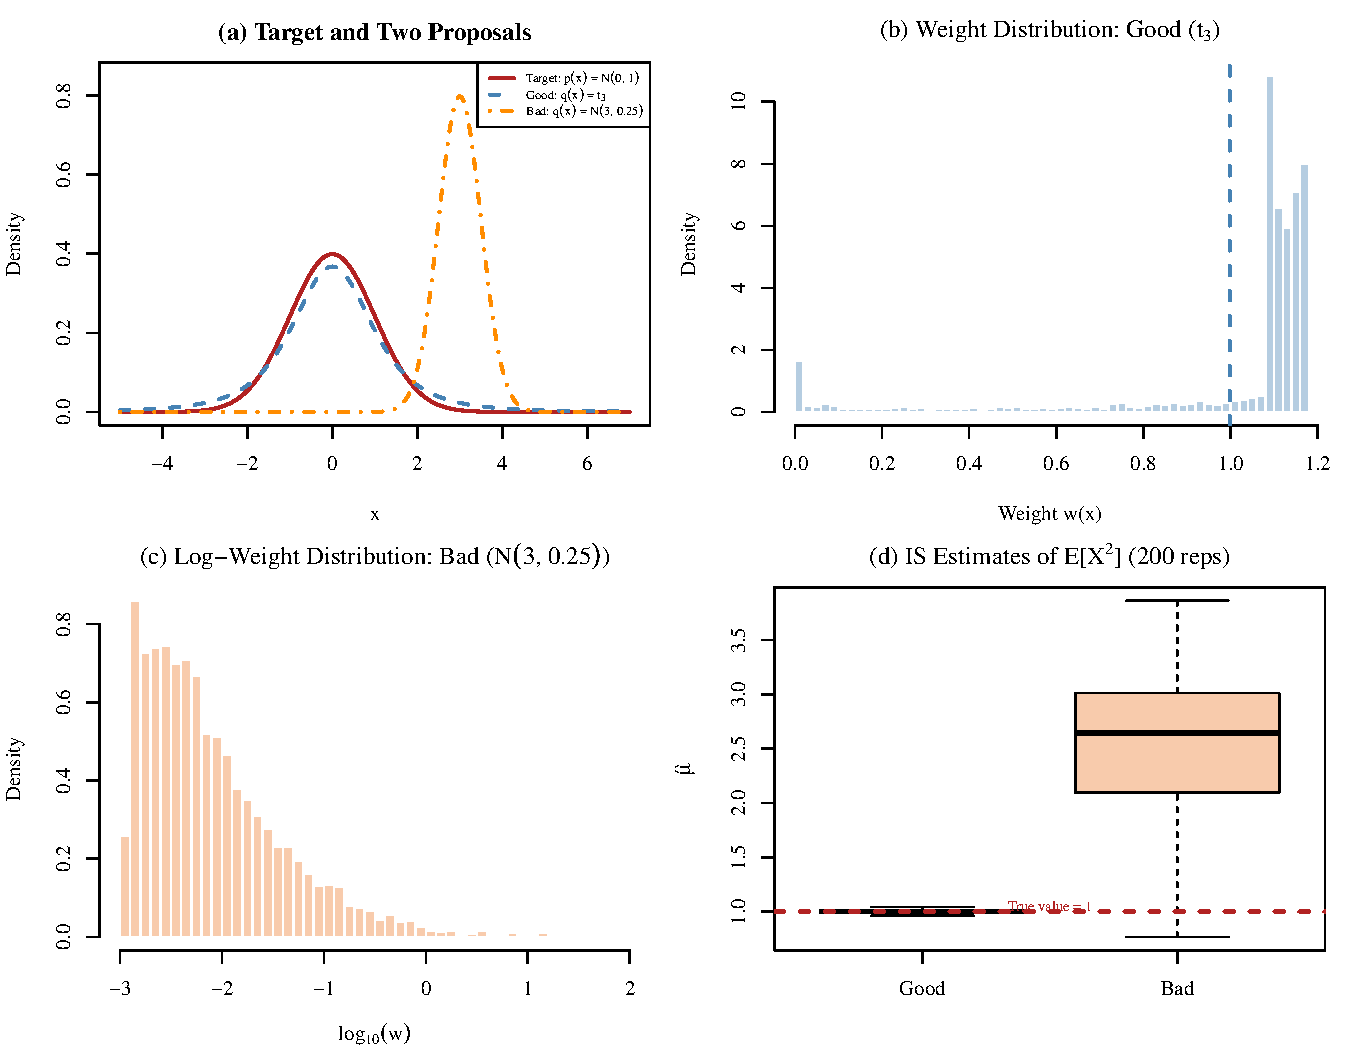
\includegraphics[width=\textwidth]{plots/fig_is_proposal_choice.pdf}
  \caption{%
    \textbf{(a)}~$N(0,1)$ target with the $t_3$ (good) and $N(3,0.25)$ (bad) proposals.
    \textbf{(b)}~Weights from $t_3$: well-concentrated.
    \textbf{(c)}~Log-weights from $N(3,0.25)$: extremely skewed.
    \textbf{(d)}~Boxplots over 200 replications; the bad proposal gives high-variance estimates.
  }
  \label{fig:proposal}
\end{figure}

% ----------------------------------------------------------------
\subsection{Figure~\ref{fig:ess}: ESS vs.\ Proposal Mismatch}

To isolate the effect of proposal location, we fix the target as $N(0,1)$ and sweep the proposal mean $\mu_q$ from 0 to 6 while keeping $\sigma_q = 1$.  At $\mu_q = 0$, $q = p$ and $\mathrm{ESS} = N$.  As $\mu_q$ grows, the overlap between $p$ and $q$ shrinks and ESS plummets.  This curve is a direct visualization of the ``curse of mismatch.''

\begin{lstlisting}
mu_vals <- seq(0, 6, length.out = 50)
for (j in seq_along(mu_vals)) {
  x_tmp <- rnorm(n_ess, mean = mu_vals[j], sd = 1)
  w_tmp <- dnorm(x_tmp) / dnorm(x_tmp, mean = mu_vals[j])
  ess_vals[j] <- (sum(w_tmp))^2 / sum(w_tmp^2)
}
\end{lstlisting}

\begin{figure}[H]
  \centering
  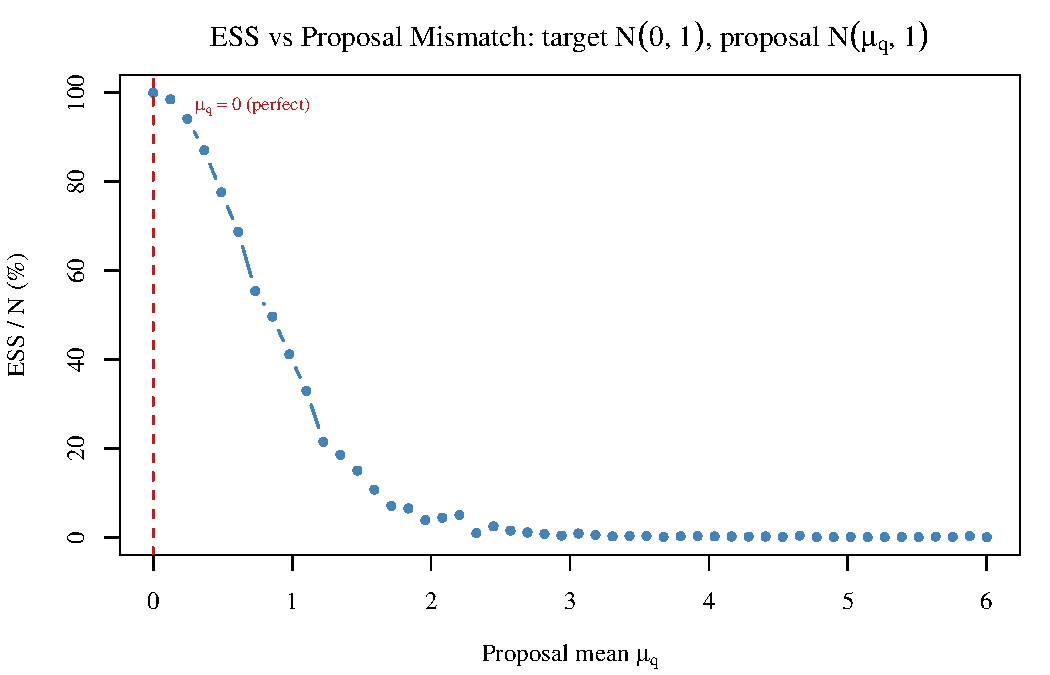
\includegraphics[width=0.75\textwidth]{plots/fig_is_ess.pdf}
  \caption{Effective sample size (as a percentage of $N$) vs.\ proposal mean $\mu_q$.  When the proposal matches the target ($\mu_q = 0$), ESS $\approx N$.  Even modest mismatch causes severe degradation.}
  \label{fig:ess}
\end{figure}

% ----------------------------------------------------------------
\subsection{Figure~\ref{fig:steps}: Step-by-Step Visualization}

The final figure isolates six sequential iterations of IS for the $\mathrm{Beta}(5,2)$/Uniform example.  For each step:
\begin{enumerate}
  \item A proposal $x$ is drawn from $q = \mathrm{Uniform}(0,1)$.
  \item Its importance weight $w = p(x)/q(x) = p(x)$ is computed.
  \item The sample is plotted on $p(x)$ with marker size proportional to $w$.
  \item The running self-normalized estimate $\hat{\mu}$ (green dashed) is updated and compared to the true mean (red dotted).
\end{enumerate}
Samples drawn near the mode of $p$ receive large weights and pull $\hat{\mu}$ toward the true value.

\begin{lstlisting}
for (k in 1:steps) {
  # draw target + proposal on [0,1]
  pt_size_k <- 0.5 + 2 * w_step[k] / max(dbeta(xgrid, a, b))
  points(x_step[k], dbeta(x_step[k], a, b),
         pch = 8, cex = 1.5 + pt_size_k * 0.5,
         col = "darkorange", lwd = 2)
  arrows(x_step[k], 0, x_step[k], dbeta(x_step[k], a, b),
         length = 0.08, col = "darkorange", lty = 3)
}
\end{lstlisting}

\begin{figure}[H]
  \centering
  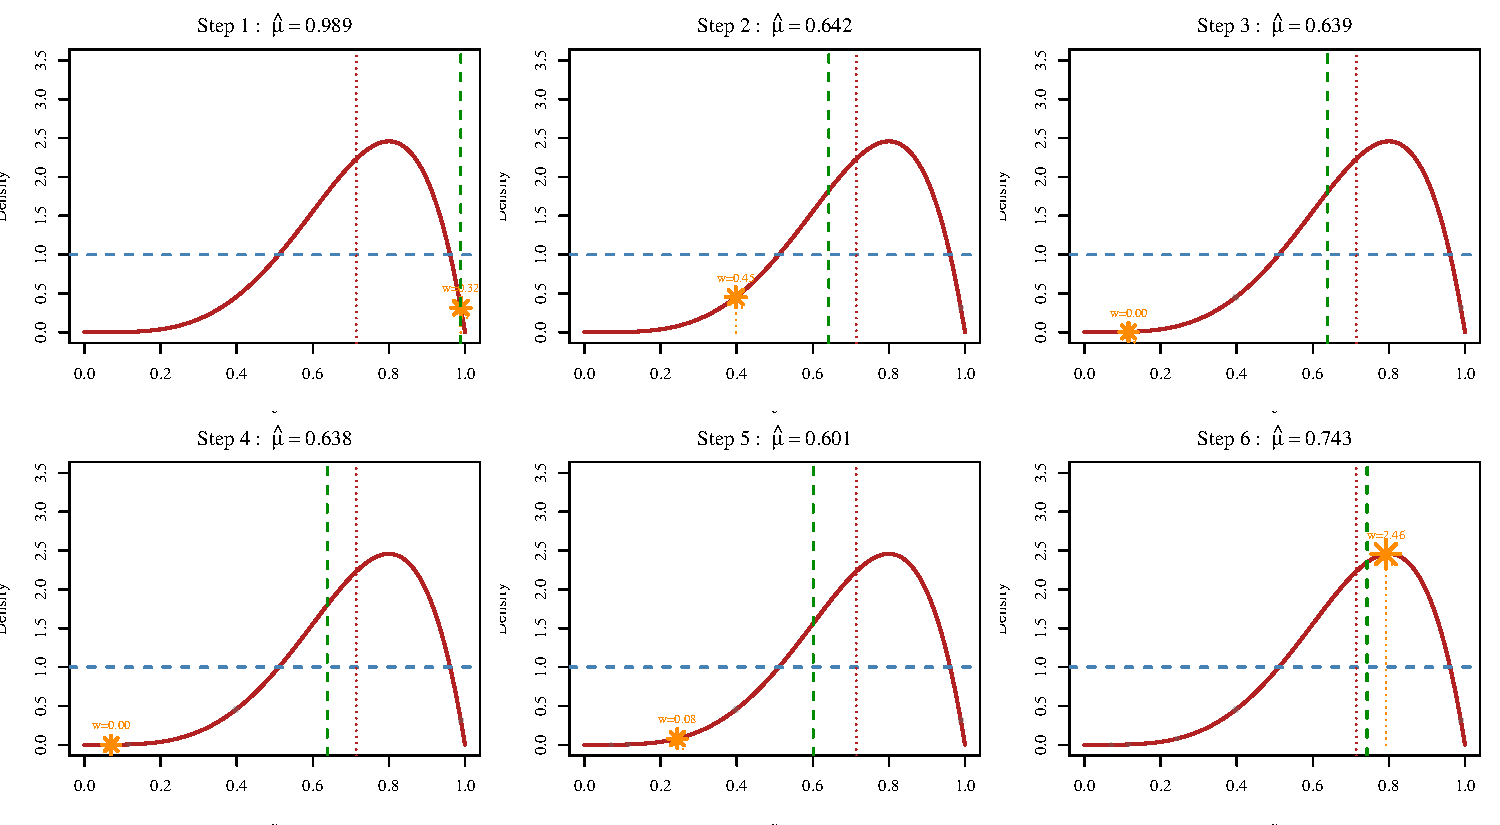
\includegraphics[width=\textwidth]{plots/fig_is_steps.pdf}
  \caption{Six sequential iterations of importance sampling for $\mathrm{Beta}(5,2)$ with a Uniform proposal.  Stars mark the current draw (size $\propto$ weight), arrows show projected height onto $p(x)$.  The green dashed line tracks the running weighted estimate $\hat{\mu}$; the red dotted line is the true mean $5/7$.}
  \label{fig:steps}
\end{figure}

% ----------------------------------------------------------------
\section{The 2D Picture: Contour Visualization}

To see importance sampling geometrically, consider a 2D target $p(\mathbf{x}) = N\!\left(\begin{smallmatrix}1\\1\end{smallmatrix}, \begin{smallmatrix}1 & 0.7 \\ 0.7 & 1\end{smallmatrix}\right)$ with a broad proposal $q(\mathbf{x}) = N(\mathbf{0},\,2I_2)$.

\paragraph{Figure~\ref{fig:contour2d}(a): Weighted samples.}
Samples are drawn from $q$ but colored and sized by their importance weight $w = p(\mathbf{x})/q(\mathbf{x})$.  High-weight points (large, red) cluster where the target (red contours) has high density but the proposal (blue dashed contours) is relatively thin.  Low-weight points (small, gray) fill the outskirts where $q$ samples freely but $p$ assigns little mass.

\paragraph{Figure~\ref{fig:contour2d}(b): Weight surface.}
A filled contour of the weight function $w(x_1, x_2)$ reveals the mismatch landscape.  The peak of $w$ is shifted away from the target's mode, reflecting how proposal concentration affects the reweighting.

\begin{figure}[H]
  \centering
  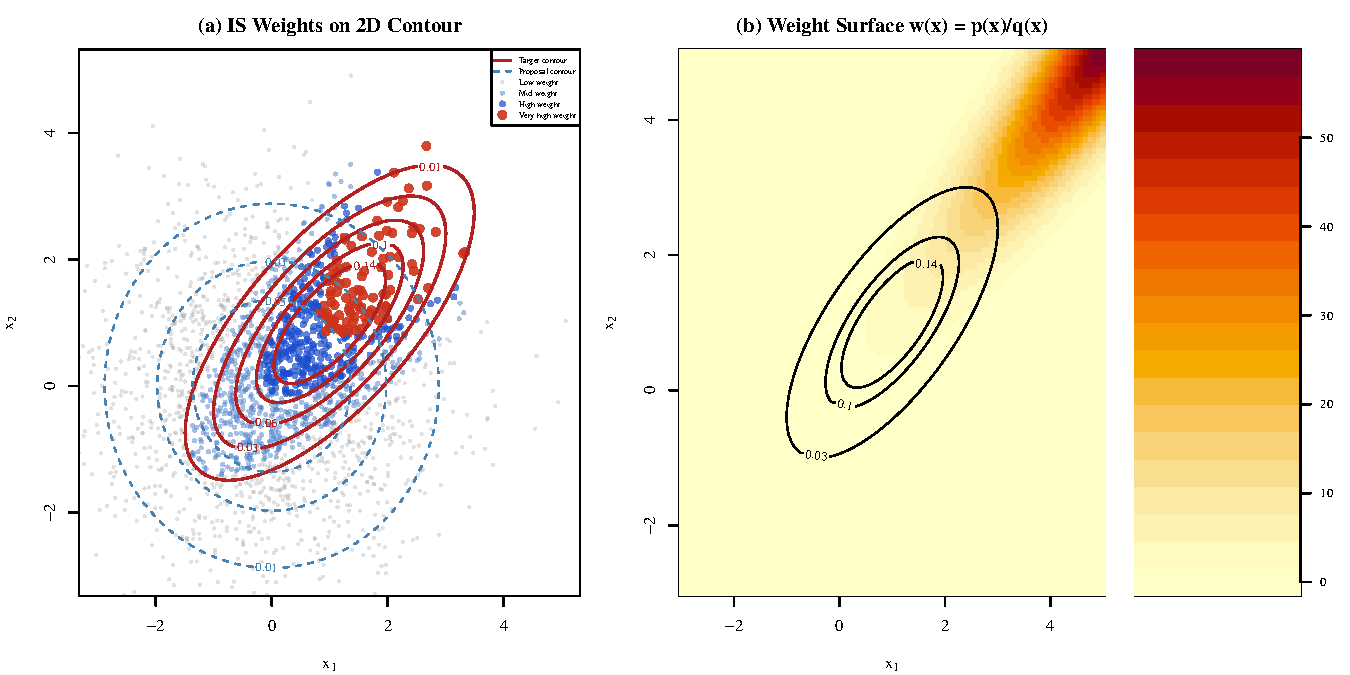
\includegraphics[width=\textwidth]{plots/fig_is_contour_2d.pdf}
  \caption{%
    \textbf{(a)}~IS applied to a correlated bivariate normal target (red contours) using a broad $N(\mathbf{0}, 2I)$ proposal (blue dashed contours).  Points are sized/colored by importance weight.
    \textbf{(b)}~Heat map of the weight surface $w(\mathbf{x}) = p(\mathbf{x})/q(\mathbf{x})$, with target contours overlaid in black.
  }
  \label{fig:contour2d}
\end{figure}

% ----------------------------------------------------------------
\section{Where Importance Sampling Fails}

\subsection{Failure Mode: Infinite Variance (Light-Tailed Proposal)}

If the proposal $q$ has \textbf{lighter tails} than the target $p$, the weight function $w(x) = p(x)/q(x)$ can grow without bound, and the variance of the IS estimator can be \textbf{infinite}---even though the estimator is formally unbiased.

\paragraph{Example.}
Let $p(x) = \mathrm{Cauchy}(0,1)$ and $q(x) = N(0,1)$.  As $|x| \to \infty$,
\[
  w(x) = \frac{p(x)}{q(x)} = \frac{(1/\pi)(1+x^2)^{-1}}{(2\pi)^{-1/2}\,e^{-x^2/2}}
  \;\sim\; \frac{\sqrt{2\pi}}{\pi}\cdot\frac{e^{x^2/2}}{1+x^2}
  \;\to\; \infty.
\]
This means $E_q[w(X)^2] = \int p(x)^2/q(x)\,dx = \infty$, so $\mathrm{Var}(\hat\mu_N) = \infty$ for any finite~$N$.

\paragraph{What happens in practice.}
Most draws from $q$ land near zero and receive moderate weights.  Occasionally, a draw lands in the far tails where the normal density is tiny but the Cauchy density is not---producing an enormous weight that dominates the entire sum.  The resulting estimates are wildly unstable across replications.

\begin{figure}[H]
  \centering
  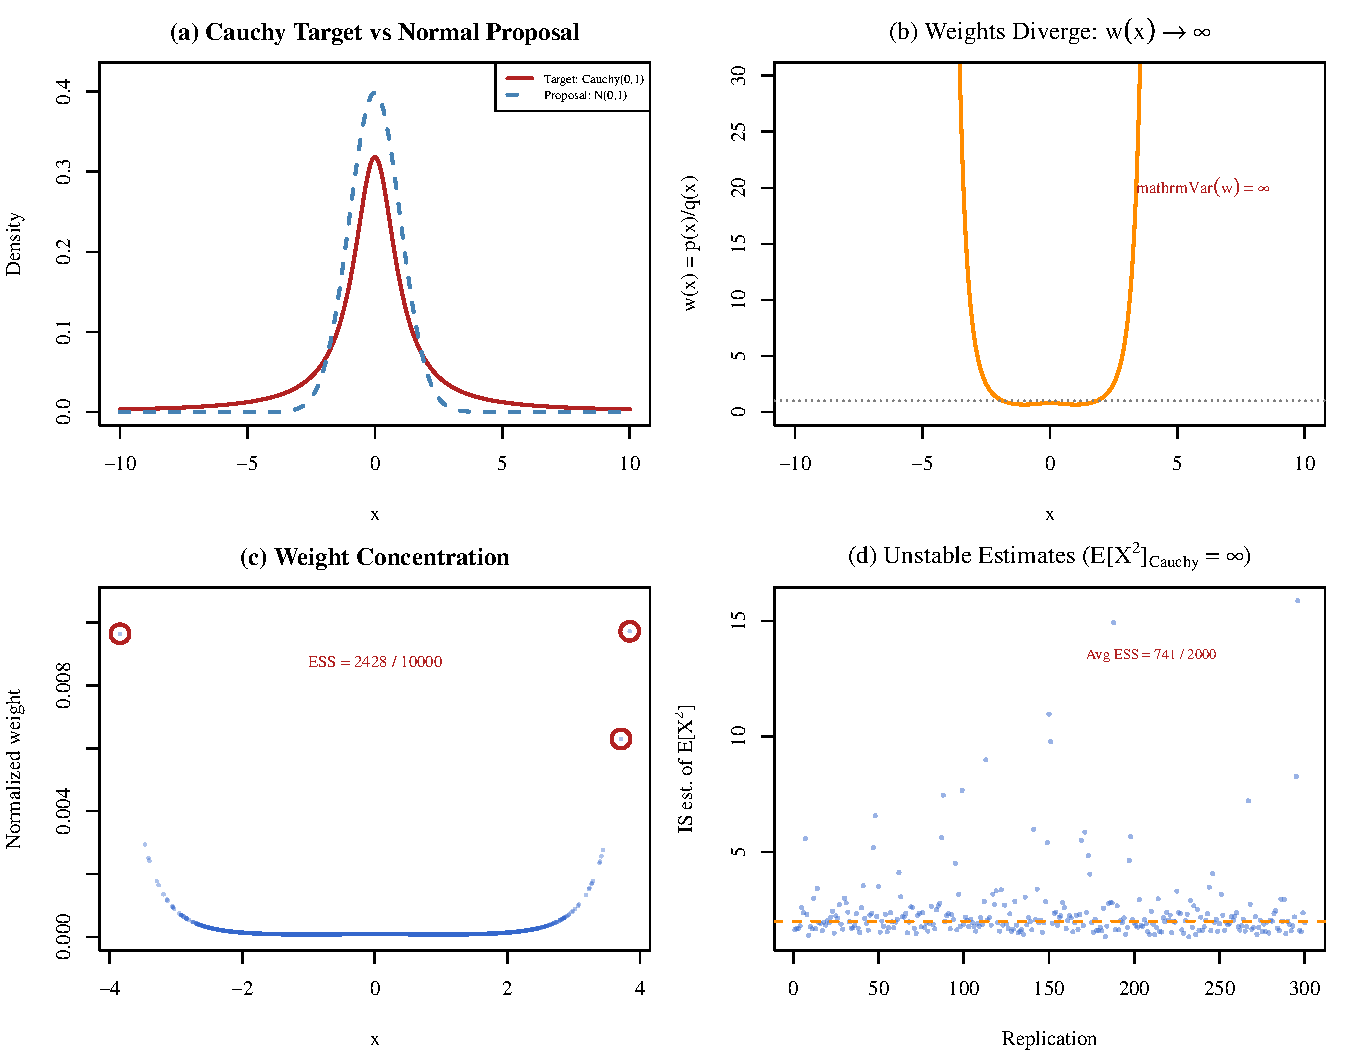
\includegraphics[width=\textwidth]{plots/fig_is_failure.pdf}
  \caption{%
    \textbf{(a)}~The Cauchy target has much heavier tails than the $N(0,1)$ proposal.
    \textbf{(b)}~The weight ratio $w(x) = p(x)/q(x)$ diverges in the tails.
    \textbf{(c)}~In a single run, a few extreme weights dominate (circled); ESS is tiny.
    \textbf{(d)}~Over 300 replications, IS estimates of $E[X^2]$ (which is $\infty$ for a Cauchy) are wildly unstable.
  }
  \label{fig:is-failure}
\end{figure}

\paragraph{Diagnostic and fix.}
A low ESS (relative to $N$) is the telltale sign.  The fix is to use a proposal with \emph{heavier} tails than the target (e.g., use a $t$-distribution or Cauchy as proposal for a normal target), or to switch to MCMC / SIR if the tails are poorly understood.

% ----------------------------------------------------------------
\section{Sampling Importance Resampling (SIR)}

Importance sampling produces \emph{weighted} samples: a set of points $\{x_i\}$ each carrying a weight $\tilde{w}_i$.  Many downstream algorithms (posterior summaries, credible intervals, predictions) are easier with \emph{unweighted} i.i.d.-like samples.  \textbf{Sampling Importance Resampling} (SIR), introduced by Rubin (1987) and discussed in BDA3 Section~10.4, bridges this gap.

\subsection{The SIR Algorithm}

\begin{algorithm}[H]
\caption{Sampling Importance Resampling (SIR)}
\label{alg:sir}
\begin{algorithmic}[1]
\For{$i = 1, \ldots, N$}
  \State Draw $X^{(i)} \sim q$ \Comment{proposal draws}
  \State Compute weight $w^{(i)} = \tilde{p}(X^{(i)}) / q(X^{(i)})$
\EndFor
\State Normalize: $\tilde{w}^{(i)} = w^{(i)} / \sum_j w^{(j)}$
\State \textbf{Resample} $M$ draws from $\{X^{(1)}, \ldots, X^{(N)}\}$ with replacement, \par with probabilities $\{\tilde{w}^{(1)}, \ldots, \tilde{w}^{(N)}\}$
\State \Return the $M$ resampled draws (now approximately i.i.d.\ from $p$)
\end{algorithmic}
\end{algorithm}

\subsection{Why It Works}

The resampling step duplicates high-weight particles and discards low-weight ones, converting a weighted sample into an approximately unweighted one.  As $N \to \infty$ (with $M$ fixed or $M/N \to 0$), the resampled draws become exactly i.i.d.\ from $p$.

For finite $N$, the quality of the resampled draws depends on the ESS of the importance weights.  If ESS is large, many distinct particles are resampled and the approximation is good.  If ESS is small, the same few high-weight particles get duplicated many times, and the resampled set contains many ties---reducing the effective diversity.  The key tradeoff: SIR converts a weighted approximation (biased toward $q$) into an unweighted approximation (biased by resampling noise).

\subsection{Code Walkthrough}

\paragraph{SIR Example 1: Beta(5,2).}
We draw $N = 10{,}000$ proposals from $\mathrm{Uniform}(0,1)$, weight by $w_i = p(x_i)$, and resample $M = 1{,}000$:

\begin{lstlisting}
x_sir <- runif(N_sir)
w_sir <- dbeta(x_sir, a, b)
w_sir_norm <- w_sir / sum(w_sir)
idx_sir <- sample(1:N_sir, size = M_sir,
                  replace = TRUE, prob = w_sir_norm)
x_resampled <- x_sir[idx_sir]
\end{lstlisting}

The resampled histogram (Figure~\ref{fig:sir}(a)) closely matches the $\mathrm{Beta}(5,2)$ density---these are now unweighted samples.

\paragraph{SIR Example 2: Bimodal mixture.}
The target $p(x) = 0.3\,N(-2,\,0.25) + 0.7\,N(2,\,0.64)$ is a mixture of two normals.  A broad $N(0,9)$ proposal covers both modes.  SIR recovers the bimodal shape faithfully (Figure~\ref{fig:sir}(b)).

\begin{figure}[H]
  \centering
  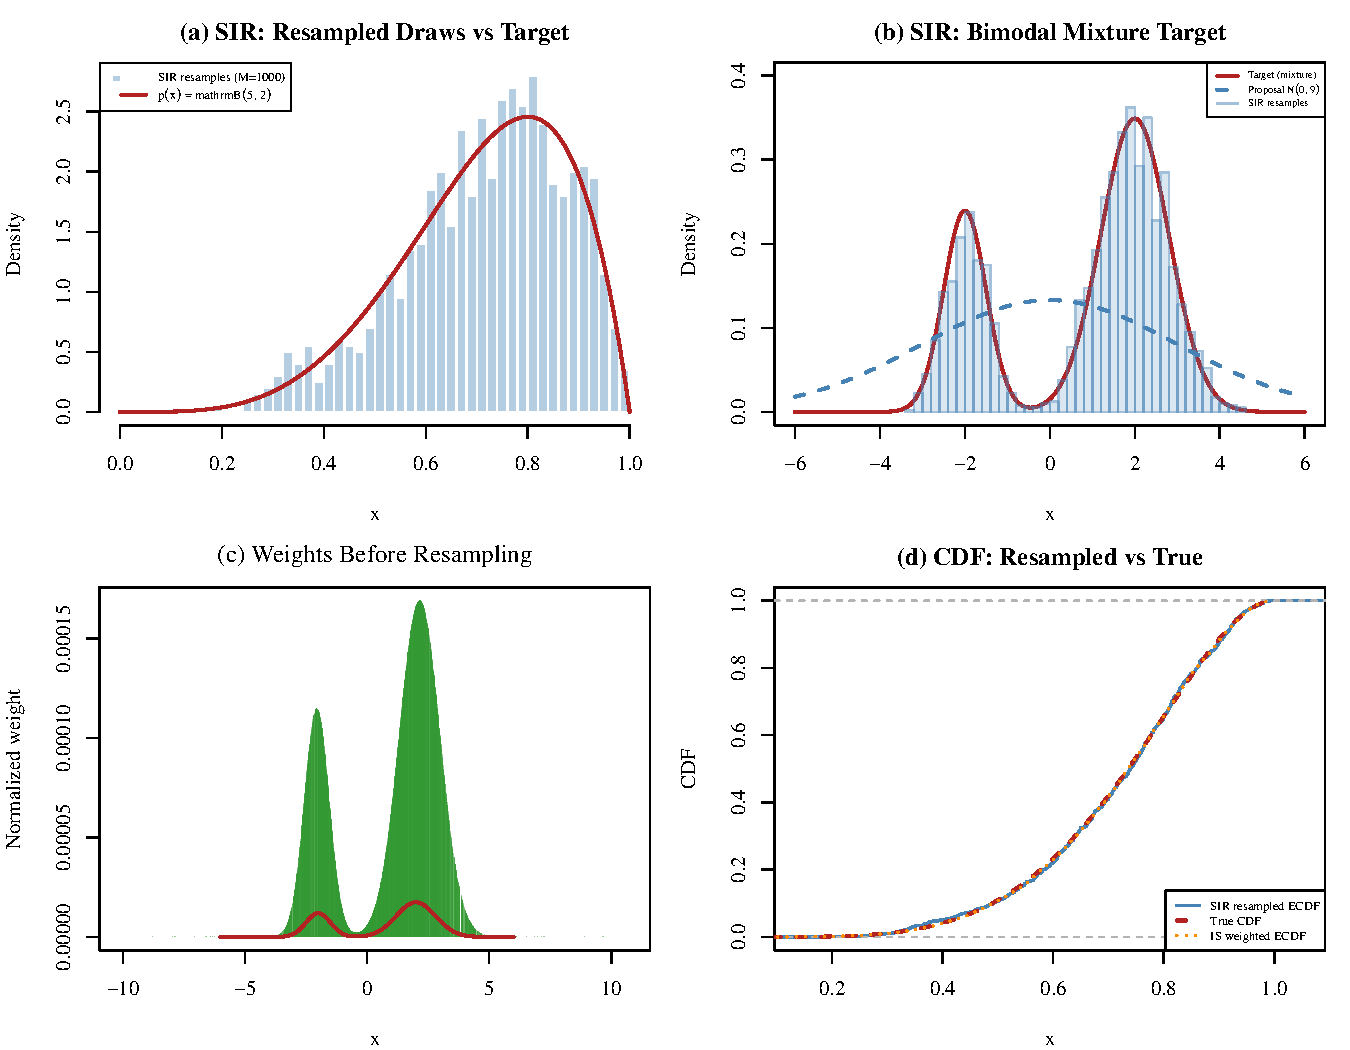
\includegraphics[width=\textwidth]{plots/fig_sir.pdf}
  \caption{%
    \textbf{(a)}~SIR resampled draws (blue histogram) vs.\ true $\mathrm{Beta}(5,2)$ density.
    \textbf{(b)}~SIR applied to a bimodal mixture target (red) using a broad $N(0,9)$ proposal (blue dashed); the resampled histogram captures both modes.
    \textbf{(c)}~Normalized weights before resampling for the bimodal example; two clusters of high weight correspond to the two modes.
    \textbf{(d)}~CDF comparison: the resampled ECDF (blue), IS weighted ECDF (orange dashed), and true CDF (red) are nearly indistinguishable.
  }
  \label{fig:sir}
\end{figure}

\subsection{How Many Resamples?}

The precision of SIR improves with resample size~$M$, but is ultimately capped by the ESS of the importance weights---resampling more than ESS copies adds diminishing returns (repeated particles).  Figure~\ref{fig:sir-conv} shows that the standard deviation of the SIR mean estimate decreases roughly as $1/\sqrt{M}$, but saturates once $M$ approaches the effective sample size from the IS step.

\begin{figure}[H]
  \centering
  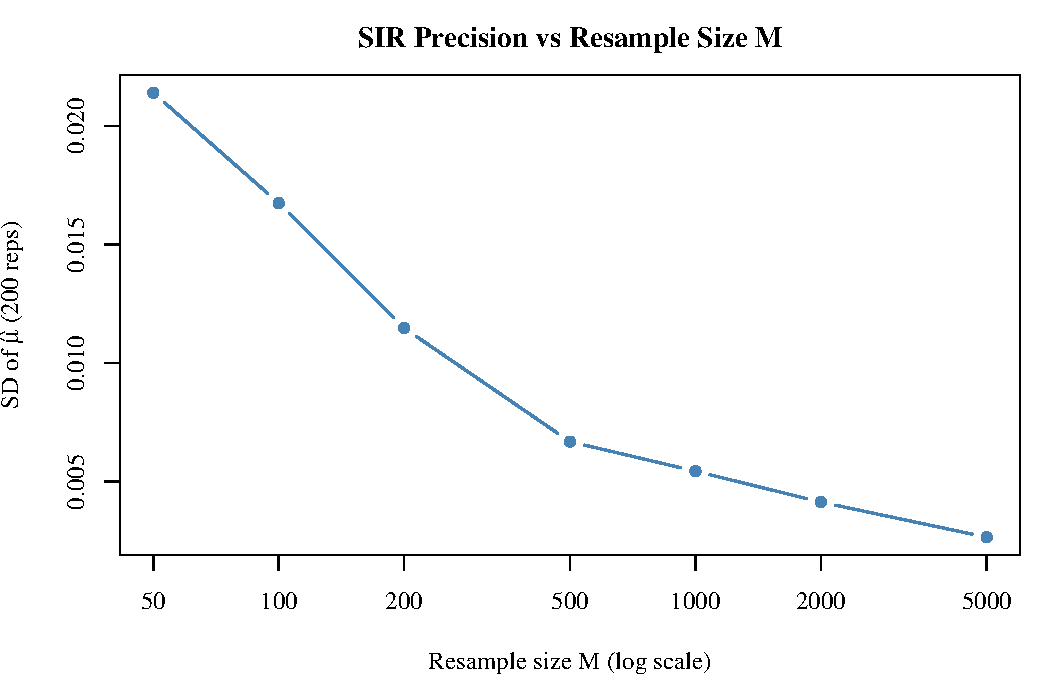
\includegraphics[width=0.75\textwidth]{plots/fig_sir_convergence.pdf}
  \caption{Standard deviation of SIR mean estimates (over 200 replications) vs.\ resample size $M$ for the $\mathrm{Beta}(5,2)$/Uniform example with $N=10{,}000$ proposals.}
  \label{fig:sir-conv}
\end{figure}

% ----------------------------------------------------------------
\section{Comparison with Rejection Sampling}

\begin{table}[H]
\centering
\begin{tabular}{lcc}
\toprule
& \textbf{Rejection Sampling} & \textbf{Importance Sampling} \\
\midrule
Samples used & Only accepted draws & All draws (reweighted) \\
Requires bounding $c$ & Yes ($c \cdot g \ge f$) & No \\
Output & Unweighted i.i.d.\ samples & Weighted samples \\
Normalizing constant & Must know $f$ exactly & Can handle $\tilde{p} \propto p$ \\
Efficiency measure & Acceptance rate $= 1/c$ & ESS / $N$ \\
High-dimensional & Fails (exponential waste) & Degrades (weight collapse) \\
\bottomrule
\end{tabular}
\caption{Rejection sampling vs.\ importance sampling at a glance.}
\label{tab:compare}
\end{table}

% ----------------------------------------------------------------
\section{Key Takeaways}

\begin{itemize}
  \item Importance sampling \textbf{reweights} draws from a proposal~$q$ to estimate expectations under a target~$p$, using every sample (no rejection).
  \item The \textbf{importance weight} $w(x) = p(x)/q(x)$ corrects for the mismatch between $q$ and $p$.
  \item The \textbf{self-normalized estimator} $\tilde{\mu}_N = \sum \tilde{w}_i h(x_i)$ handles unnormalized targets, which is essential in Bayesian computation where the posterior is known only up to a constant.
  \item A good proposal must have \textbf{heavier tails} than the target in regions where $|h(x)\,p(x)|$ is large.  If $q$ has lighter tails than $p$, the variance of $\hat{\mu}$ can be \emph{infinite}.
  \item The \textbf{effective sample size} (ESS) diagnoses proposal quality.  Low ESS means a few samples dominate the estimate---the sampler has effectively ``wasted'' most of its draws.
  \item IS is especially powerful for \textbf{rare-event estimation}, where it can improve efficiency by orders of magnitude over naive MC.
  \item \textbf{SIR} converts weighted IS samples into approximately i.i.d.\ draws by resampling with replacement proportional to weights.  This is the workhorse behind particle filters and practical Bayesian computation.
  \item In \textbf{high dimensions}, finding a $q$ with good overlap becomes exponentially harder---motivating sequential Monte Carlo (particle filters) and MCMC methods.
\end{itemize}

\end{document}
